%% Robustness indices reward poor nominal schedules
%% Elsevier CAS single-column template (cas-sc) — submission format
%% Target: Computers & Industrial Engineering

\documentclass[a4paper,fleqn]{cas-sc}

\usepackage[authoryear,longnamesfirst]{natbib}
\usepackage{amsmath,amssymb,amsthm}
\usepackage{booktabs}
\usepackage{multirow}
\usepackage{pifont}
\usepackage{graphicx}
\usepackage[english]{babel}

\newtheorem{proposition}{Proposition}
\newtheorem{corollary}{Corollary}
\newdefinition{definition}{Definition}
\newproof{pf}{Proof}

\newcommand{\NRegimes}{9}
\newcommand{\NRunsDisrupted}{4{,}500}
\newcommand{\NInstances}{43}
\newcommand{\NConfRegimes}{6}
\newcommand{\NDescRegimes}{3}
\newcommand{\RhoConfMin}{\ensuremath{-0.985}}
\newcommand{\RhoConfMax}{\ensuremath{-0.948}}
\newcommand{\RhoConfMedian}{\ensuremath{-0.948}}
\newcommand{\PConfMax}{\ensuremath{3\times10^{-5}}}
\newcommand{\RhoDesc}{\ensuremath{-0.800}}
\newcommand{\NRhoNegative}{9}
\newcommand{\NDisagree}{9}
\newcommand{\PenaltyMin}{15.8}
\newcommand{\PenaltyMax}{49.3}
\newcommand{\PenaltyMedian}{25.7}
\newcommand{\TauMin}{\ensuremath{-0.60}}
\newcommand{\TauMax}{\ensuremath{-0.29}}
\newcommand{\NRLNotWorse}{9}
\newcommand{\NRLBest}{5}
\newcommand{\FriedmanPMax}{\ensuremath{6.7\times10^{-28}}}
\newcommand{\ArrCD}{0.79}
\newcommand{\ArrRankMin}{1.57}
\newcommand{\ArrRankMax}{1.62}
\newcommand{\ArrGapMin}{0.11}
\newcommand{\ArrGapMax}{0.20}
\newcommand{\CRWins}{6}
\newcommand{\LWKRWins}{3}
\newcommand{\CompGlobal}{233.4}
\newcommand{\CompFamily}{132.4}
\newcommand{\CompOracle}{7.6}
\newcommand{\CompPMax}{\ensuremath{4.1\times10^{-5}}}
\newcommand{\PropCells}{150}
\newcommand{\PropErr}{\ensuremath{9.4\times10^{-6}}}
\newcommand{\PctRINeg}{65}
\newcommand{\NRINeg}{97}
\newcommand{\QCpsat}{42.0}
\newcommand{\QGa}{41.3}
\newcommand{\QMor}{44.1}
\newcommand{\QMwkr}{46.8}
\newcommand{\QRl}{48.0}
\newcommand{\WallGa}{30}
\newcommand{\WallCpsat}{0.046}
\newcommand{\WallRl}{0.095}
\newcommand{\PRlCpsat}{0.375}
\newcommand{\PRlGa}{0.250}
\newcommand{\NEffOffline}{4}
\newcommand{\NExcludedArr}{5}
\newcommand{\CVaRTail}{3}
\newcommand{\SeedsPerCell}{30}
\newcommand{\CliqueArr}{1}
\newcommand{\CliqueOther}{3}
\newcommand{\NomRlTwo}{18.4}
\newcommand{\NomCrTwo}{220.1}
\newcommand{\NomRlAll}{24.8}
\newcommand{\NomCrAll}{430.3}
\newcommand{\NomMwkrTwo}{30.7}

\newcommand{\Cmax}{C_{\max}}
\newcommand{\RI}{\mathrm{RI}}
\newcommand{\RQ}{\mathrm{RQ}}
\newcommand{\CVaR}{\mathrm{CVaR}}

\begin{document}
\let\WriteBookmarks\relax
\def\floatpagepagefraction{1}
\def\textpagefraction{.001}

\shorttitle{Robustness indices reward poor nominal schedules}
\shortauthors{J. J. Sánchez Acuña}

\title[mode=title]{Robustness indices reward poor nominal schedules: a
measurement audit of dynamic job-shop scheduling under disruption}

\author[1]{Joseph Javier Sánchez Acuña}
\cormark[1]
\ead{joseph.sanchez@uniminuto.edu.co}
\credit{Conceptualization, Methodology, Software, Formal analysis,
Investigation, Data curation, Writing -- original draft,
Writing -- review \& editing, Visualization}

\affiliation[1]{organization={Universidad de los Andes},
                city={Bogotá},
                country={Colombia}}

\cortext[1]{Corresponding author.}

\begin{abstract}
Deep reinforcement learning (DRL) is increasingly proposed for dynamic
job-shop scheduling on the grounds that learned dispatching policies are more
\emph{robust} to disruption than offline optimisation. That claim is almost
always supported by a robustness index of the form
$\RI=(\mathbb{E}[\Cmax^{\text{pert}}]-\Cmax^{\text{nom}})/\Cmax^{\text{nom}}$,
which normalises the degradation a method suffers by its own undisrupted
makespan. We show, analytically and empirically, that this self-referential
normalisation makes the index unusable for comparing methods. Writing $r$ and
$q$ for the relative deviations of the nominal and the realised makespan from a
certified optimum, we prove that $\RI=(q-r)/(1+r)$, so that at equal realised
performance $\RI$ is strictly decreasing in $r$: the worse a method's nominal
schedule, the more robust it appears. In a corpus of \NRunsDisrupted{} disrupted
executions spanning \NRegimes{} pre-registered regimes across three disruption
classes, $\RI$ is rank-correlated with nominal deviation in every regime, at
$\rho_s$ between \RhoConfMin{} and \RhoConfMax{} ($p\le\PConfMax{}$) across the
\NConfRegimes{} regimes that compare ten methods, and the ordering it induces
disagrees with the ordering by realised quality in all \NRegimes{} (Kendall
$\tau$ negative throughout). Selecting a scheduler by $\RI$ rather than
by realised quality costs between \PenaltyMin{} and \PenaltyMax{} percentage
points of deviation from the optimum (median \PenaltyMedian{}). We propose
realised quality --- the deviation of the executed makespan from the certified
optimum --- together with its $\CVaR_{90}$ tail, and a three-comparator
reporting discipline that separates the mean rule, the best rule per family and
the per-instance oracle. Re-measured this way, a heterogeneous
graph-neural-network PPO policy is statistically indistinguishable from the best
comparator in all \NRegimes{} regimes and ranks first in \NRLBest{}, including
all three dynamic-arrival regimes --- a conclusion the conventional index
inverts.
\end{abstract}

\begin{highlights}
\item The conventional schedule robustness index is proved to be a strictly
decreasing function of nominal deviation at fixed realised performance.
\item It correlates with nominal deviation in all nine disruption regimes, at
$\rho_s=-0.95$ to $-0.98$ where ten methods are compared: worse nominal
schedules score as more robust.
\item Ranking by the index contradicts ranking by realised quality in all nine
regimes, costing up to 49.3 percentage points of deviation from the optimum.
\item Realised quality against a certified optimum, plus a $\CVaR_{90}$ tail,
restores cross-method comparability without new experiments.
\item Under the corrected metric a GNN--PPO policy matches the best comparator
in every regime and ranks first in five, including all arrival regimes.
\end{highlights}

\begin{keywords}
Dynamic job-shop scheduling \sep Robustness measurement \sep
Deep reinforcement learning \sep Graph neural networks \sep
Constraint programming \sep Experimental methodology
\end{keywords}

\maketitle

% ===========================================================================
\section{Introduction}\label{sec:intro}

Production schedules are computed under assumptions that the shop floor does not
honour. Machines break down, processing times realise away from their estimates,
and jobs arrive after the schedule has been fixed. The scheduling literature has
responded with two broad strategies: compute a schedule offline and repair it as
events unfold, or learn a dispatching policy that decides online and therefore
never commits to a sequence it must later abandon
\citep{ouelhadj2009,aytug2005}. The second strategy has attracted intense
recent interest, with graph neural networks supplying a size-agnostic state
representation and policy-gradient methods supplying the learning signal
\citep{zhang2020,park2021,song2023,bengio2021}.

The empirical case for learned policies rests on a robustness claim. A learned
policy is said to degrade less under disruption than an offline optimum does,
and this is quantified by an index that compares a method's disrupted makespan
to its own undisrupted makespan:
\begin{equation}\label{eq:ri-intro}
  \RI \;=\; \frac{\mathbb{E}\!\left[\Cmax^{\text{pert}}\right]-\Cmax^{\text{nom}}}
                 {\Cmax^{\text{nom}}}.
\end{equation}
Variants of \eqref{eq:ri-intro} appear throughout the robust-scheduling
literature \citep{leon1994,mehta1998,goren2008,sabuncuoglu2000} and have been
carried into the DRL-scheduling literature largely unexamined
\citep{smit2025,huang2025,xu2024survey}. The index has an appealing reading: it
is dimensionless, it is comparable across instances of different size, and a
value near zero says that disruption cost the method little.

This paper argues that \eqref{eq:ri-intro} cannot bear the comparative weight
placed on it, and that the problem is structural rather than a matter of
estimation noise. The denominator is the method's own nominal makespan. A method
that produces a poor nominal schedule is therefore graded against a lenient
reference, and one that produces a near-optimal schedule is graded against a
demanding one. Section~\ref{sec:framework} makes this exact: with $r$ the
relative deviation of the nominal makespan from a certified optimum and $q$ the
relative deviation of the realised makespan from the same optimum,
$\RI=(q-r)/(1+r)$, whose partial derivative in $r$ is strictly negative. Two
methods that deliver \emph{identical} executed schedules are ranked by $\RI$ in
reverse order of the quality of the plans they started from.

The consequence is not hypothetical. We re-analyse a pre-registered corpus of
\NRunsDisrupted{} disrupted executions covering three disruption classes at three
severities each --- machine breakdowns, stochastic processing times and dynamic
job arrivals --- for nine priority dispatching rules and a heterogeneous
GNN--PPO policy, together with \NInstances{} nominal instances with proven
optima. In every one of the \NRegimes{} regimes, $\RI$ is negatively
rank-correlated with how bad the nominal schedule was --- almost perfectly so in
the \NConfRegimes{} regimes that compare ten methods --- and the method it
nominates as most robust is never the method that actually finishes closest to
the optimum. Under breakdowns and stochastic processing times the index crowns
the critical-ratio rule, whose nominal schedules sit some $220\%$ above the
optimum; under dynamic arrivals it crowns least-work-remaining, at $187\%$. Both
are among the worst performers once the executed schedule is measured against a
fixed reference.

\paragraph{Contributions.} This paper makes four.
\begin{enumerate}[(i)]
\item \textbf{An analytic characterisation of the failure mode.}
Proposition~\ref{prop:ri} decomposes $\RI$ into nominal and realised deviation
and shows the monotone dependence on the former; Corollary~\ref{cor:neg}
identifies negative $\RI$ --- routinely reported as strong robustness --- as the
signature of a nominal schedule so poor that perturbation improves it in
expectation.
\item \textbf{A quantification of the resulting decision error.} Across
\NRegimes{} regimes, ranking by $\RI$ and ranking by realised quality disagree
without exception, and acting on the former costs \PenaltyMin{}--\PenaltyMax{}
percentage points of deviation from the optimum.
\item \textbf{A corrected measurement protocol.} Realised quality against a
certified optimum, reported jointly with a $\CVaR_{90}$ tail and against three
explicitly separated dispatching comparators, restores cross-method
comparability. The protocol requires no additional experiments: it is a
re-measurement of runs already performed.
\item \textbf{A re-evaluation of the learned policy under that protocol.} The
GNN--PPO policy is not significantly worse than the best-ranked comparator in
any of the \NRegimes{} regimes at the Nemenyi critical difference and ranks
first in \NRLBest{}, including all three dynamic-arrival regimes --- while the
conventional index places it near the bottom. We are careful throughout to read
a failure to reject as a tie rather than as a win.
\end{enumerate}

Section~\ref{sec:related} situates the argument. Section~\ref{sec:problem}
fixes the problem and the disruption model. Section~\ref{sec:framework} develops
the measurement framework. Section~\ref{sec:design} describes the experimental
design and the pre-registration that governs it. Section~\ref{sec:results}
reports the audit. Section~\ref{sec:discussion} discusses implications and
limitations, and Section~\ref{sec:conclusion} concludes.

% ===========================================================================
\section{Related work}\label{sec:related}

\subsection{Learning to schedule}

Dispatching rules remain the operational default in dynamic shops because they
are cheap, interpretable and require no state beyond what the shop already
tracks \citep{haupt1989,holthaus1997}. Their weakness is that no single rule
dominates: performance depends on shop load, due-date tightness and the
disruption regime. Learning a dispatching policy is an attempt to obtain the
online character of a rule with the instance-adaptivity of search.
\citet{zhang2020} framed job-shop scheduling as sequential decision making over
a disjunctive graph and learned a policy with proximal policy optimisation
\citep{schulman2017}; \citet{park2021} and \citet{song2023} extended the idea to
richer graph encodings and to the flexible variant. Recent surveys
\citep{kayhan2023,smit2025,huang2025,xu2024survey} document rapid growth in the
area and, notably, converge on the observation that evaluation practice is
heterogeneous enough to make cross-paper comparison difficult.

\subsection{Robustness measurement in scheduling}

Robust scheduling distinguishes \emph{robustness} --- retained solution quality
under realisation --- from \emph{stability}, the degree to which the executed
schedule resembles the planned one \citep{leon1994,goren2008}. Both are usually
measured relative to the method's own plan. \citet{leon1994} define robustness
through the expected makespan increase relative to the deterministic schedule;
\citet{mehta1998} measure predictability similarly; \citet{sabuncuoglu2000} and
\citet{aytug2005} survey the reactive-scheduling variants of the same
construction. \citet{herroelen2005} note in the project-scheduling context that
such measures conflate the quality of the baseline with its resilience, but the
observation has not propagated into machine-scheduling evaluation practice, and
in particular not into the DRL-scheduling literature, where the index is
typically inherited without an examination of what its denominator does.

Our contribution here is to make that conflation precise and to show that it is
not a second-order concern: in the regimes we study it is the dominant term, and
it inverts the induced ordering.

\subsection{Evaluation hygiene in learning-based methods}

The reproducibility literature in reinforcement learning has repeatedly found
that reported gains are sensitive to seeds, to the choice of baseline and to the
statistical procedure \citep{henderson2018,agarwal2021}. The remedies proposed
there --- pre-registration of hypotheses, explicit comparator definitions,
distribution-free tests over instance sets, and reporting of tails rather than
means alone \citep{demsar2006,garcia2008,munafo2017,kerr1998} --- transfer
directly to scheduling, where the instance set plays the role of the task
distribution. This paper applies them, and adds one scheduling-specific
requirement: the reference against which quality is measured must be external to
the method being graded.

% ===========================================================================
\section{Problem setting}\label{sec:problem}

\subsection{The dynamic flexible job-shop problem}

An instance comprises a set of jobs $\mathcal{J}=\{J_1,\dots,J_n\}$ and machines
$\mathcal{M}=\{M_1,\dots,M_m\}$. Job $J_i$ is a chain of operations
$O_{i1}\prec O_{i2}\prec\cdots\prec O_{in_i}$; operation $O_{ij}$ may be
processed on any machine in an eligibility set
$\mathcal{M}_{ij}\subseteq\mathcal{M}$, taking $p_{ijk}$ time units on
$M_k\in\mathcal{M}_{ij}$. In the classical job shop $|\mathcal{M}_{ij}|=1$ for
all $(i,j)$. Machines process one operation at a time and operations are
non-preemptable once started. A solution assigns each operation a machine and a
start time consistent with precedence and machine capacity; the objective is the
makespan $\Cmax=\max_{i}C_{i n_i}$.

The dynamic variant lets the instance change during execution. We write
$\xi$ for a realisation of the disruption process and $\Cmax^{\text{pert}}(\xi)$
for the makespan actually achieved when a method's decisions are executed
against $\xi$.

\subsection{Disruption classes}\label{sec:disruption}

Three disruption classes are modelled, each at three severities, giving the
\NRegimes{} regimes of the experimental grid. The parameterisations were fixed
before any result was observed (Section~\ref{sec:prereg}).

\paragraph{Machine breakdowns.} Each machine alternates between available and
under-repair states calibrated to a target availability
$A_k\in\{0.95,0.90,0.80\}$. Times to failure are exponential and times to repair
log-normal with shape $\sigma_{\text{TTR}}=0.5$ and a mean-time-to-repair
multiplier of $2.0$. An operation in progress when its machine fails resumes on
repair.

\paragraph{Stochastic processing times.} Realised durations are drawn as
$\tilde{p}_{ijk}=p_{ijk}\cdot\varepsilon$ with
$\varepsilon\sim\mathrm{LogNormal}$ calibrated to unit mean and coefficient of
variation $\sigma\in\{0.10,0.25,0.50\}$, so that the expected instance is
unchanged and only its dispersion varies.

\paragraph{Dynamic job arrivals.} New jobs arrive as a Poisson process whose
rate is calibrated to a target machine utilisation
$\rho\in\{0.70,0.85,0.95\}$, up to a horizon after which no further arrivals
occur.

\subsection{Execution semantics}\label{sec:execution}

The distinction between methods that decide once and methods that decide
continuously must be made explicit, because it determines what a disrupted
makespan even means.

An \emph{offline} method (constraint programming, a genetic algorithm) produces
a complete schedule against the nominal instance. Under disruption that schedule
is executed with right-shift repair: the machine sequence is preserved and start
times are pushed forward as needed to respect the realised durations,
availabilities and release dates. An \emph{online} method (a dispatching rule, a
learned policy) is invoked at each decision point against the state as it
actually is, and therefore never holds a sequence it must repair.

This asymmetry is intrinsic to the comparison and we do not attempt to remove
it. We do, however, decline to let it hide inside a metric: the measurement
framework of Section~\ref{sec:framework} grades both families against the same
external reference.

Not every dispatching rule survives the arrival regimes. \NExcludedArr{} of the
nine are excluded there, for two distinct reasons. \textsc{edd} and \textsc{cr}
require job due dates, and the due dates of jobs that did not exist when the
instance was created are not defined by the instance; synthesising them online
is a modelling decision, not an implementation detail. \textsc{spt},
\textsc{lpt} and \textsc{mwkr} require per-operation duration or
remaining-work quantities indexed against the original operation set, which the
implementation does not maintain for dynamically arriving jobs. Four rules
(\textsc{fifo}, \textsc{mor}, \textsc{lor}, \textsc{lwkr}) plus the learned
policy are therefore compared under arrivals, against ten methods elsewhere.

This restriction matters for how the arrival results should be read, and we flag
it here rather than in a footnote: \textsc{mwkr}, which outranks the learned
policy in five of the six non-arrival regimes, is among the rules excluded. The
arrival comparison is therefore against a weaker field than the breakdown and
stochastic-time comparisons, and the policy's first-place finish there is a
first place among four rules, not among nine. Section~\ref{sec:threats} returns
to this. Removing the restriction requires tracking each job's true arrival time
and recomputing rule state against a growing operation set --- a change of state
representation we did not attempt, and disclose rather than resolve.

% ===========================================================================
\section{A measurement framework}\label{sec:framework}

\subsection{The conventional index and what its denominator does}

\begin{definition}[Robustness index]\label{def:ri}
For a method producing nominal makespan $\Cmax^{\text{nom}}$ and expected
disrupted makespan $\mathbb{E}[\Cmax^{\text{pert}}]$ on the same instance,
\[
  \RI=\frac{\mathbb{E}[\Cmax^{\text{pert}}]-\Cmax^{\text{nom}}}{\Cmax^{\text{nom}}}.
\]
\end{definition}

Let $\Cmax^{\star}$ denote a certified optimum for the nominal instance and
define the two \emph{externally referenced} deviations
\begin{equation}\label{eq:rq}
  r=\frac{\Cmax^{\text{nom}}-\Cmax^{\star}}{\Cmax^{\star}},
  \qquad
  q=\frac{\mathbb{E}[\Cmax^{\text{pert}}]-\Cmax^{\star}}{\Cmax^{\star}} .
\end{equation}
Here $r$ is the familiar relative percentage deviation of the plan and $q$ is
what we will call \emph{realised quality}: how far the schedule that was
actually executed finished from the best schedule that existed for the nominal
instance. Both are measured against a reference that no method can influence.

\begin{proposition}\label{prop:ri}
With $r$ and $q$ as in \eqref{eq:rq} and $\Cmax^{\star}>0$,
\begin{equation}\label{eq:decomp}
  \RI=\frac{q-r}{1+r},
  \qquad\text{and}\qquad
  \frac{\partial \RI}{\partial r}\bigg|_{q}=-\frac{1+q}{(1+r)^{2}}<0 .
\end{equation}
\end{proposition}

\begin{pf}
Substituting $\Cmax^{\text{nom}}=\Cmax^{\star}(1+r)$ and
$\mathbb{E}[\Cmax^{\text{pert}}]=\Cmax^{\star}(1+q)$ into
Definition~\ref{def:ri} gives
$\RI=\big(\Cmax^{\star}(1+q)-\Cmax^{\star}(1+r)\big)/\Cmax^{\star}(1+r)
=(q-r)/(1+r)$. Differentiating in $r$ at fixed $q$,
$\partial\RI/\partial r=\big[-(1+r)-(q-r)\big]/(1+r)^2=-(1+q)/(1+r)^2$, which is
negative whenever $q>-1$, i.e.\ whenever the disrupted makespan is positive.
\qed
\end{pf}

\begin{corollary}[Rank inversion at equal performance]\label{cor:inv}
Two methods with identical realised quality $q$ but nominal deviations
$r_1<r_2$ satisfy $\RI_1>\RI_2$. The method with the worse plan receives the
better robustness score.
\end{corollary}

\begin{corollary}[Negative index]\label{cor:neg}
$\RI<0$ if and only if $q<r$: the expected disrupted makespan is \emph{below}
the nominal one. This can only occur when the nominal schedule was poor enough
that the disruption process, by reordering work it had sequenced badly, improves
it in expectation.
\end{corollary}

Corollary~\ref{cor:neg} deserves emphasis because negative robustness indices
are reported in the literature as evidence of exceptional resilience. Under
Definition~\ref{def:ri} they are instead a diagnostic of a bad baseline. A
method cannot benefit from machine failures; it can only have been scheduling so
inefficiently that the failures were not the binding constraint.

Proposition~\ref{prop:ri} is an identity, not an approximation. Evaluated over
the \PropCells{} (method $\times$ instance $\times$ regime) cells of our corpus,
the maximum absolute discrepancy between $\RI$ as computed from raw makespans
and $(q-r)/(1+r)$ as computed from the stored deviations is \PropErr{}; computed
from raw makespans on both sides the discrepancy falls to floating-point noise,
confirming that the residual is rounding in the recorded deviation columns.

\subsection{Realised quality}

We take $q$ of \eqref{eq:rq} as the primary performance measure under
disruption and call it realised quality, $\RQ$. It has three properties the
conventional index lacks. It is referenced externally, so a method cannot
improve its score by planning badly. It is comparable across methods, because
all methods on an instance share the denominator $\Cmax^{\star}$. And it is
comparable to the nominal deviation $r$ on the same scale, so the cost of
disruption is read as the difference $q-r$ rather than being folded into a
ratio.

It also has a limitation worth stating. $\RQ$ measures the executed schedule
against the optimum \emph{of the nominal instance}, which under dynamic arrivals
is not the optimum of the instance that was actually executed. The quantity is
therefore a lower-bound-referenced deviation rather than a true optimality gap
in the arrival regimes; it remains comparable across methods, which is what the
comparison requires, but its absolute magnitude there should not be read as an
optimality gap. We report arrival regimes separately throughout for this reason.

\subsection{Tail risk}

A mean conceals the executions a shop actually fears. We therefore report,
alongside $\mathbb{E}[\RQ]$, the conditional value at risk at the $90$th
percentile,
\begin{equation}
  \CVaR_{90}(\RQ)=\mathbb{E}\big[\RQ \mid \RQ \ge \mathrm{VaR}_{90}(\RQ)\big],
\end{equation}
the mean realised quality over those realisations at or above the $90$th
percentile \citep{rockafellar2000,jorion2007}. With \SeedsPerCell{} seeds per
(instance, method) this averages the worst \CVaRTail{} realisations, so it is a
coarse tail estimate and we read it as a direction, not a precise quantile. Two methods with equal expected performance
and different tail behaviour are operationally different, and a scheduler chosen
for a shop that cannot absorb a late finish should be chosen on the tail.

\subsection{Comparator discipline}\label{sec:comparators}

Claims of the form ``the policy beats the best dispatching rule'' are
underdetermined until \emph{best} is defined, and the available definitions do
not agree. We report all three, always separately and always labelled.

\begin{description}
\item[$\mathrm{PDR}_{\mathrm{global}}$] the mean deviation over all nine rules:
what a practitioner obtains who has not tuned rule selection.
\item[$\mathrm{PDR}_{\mathrm{family}}$] the mean, over the five behavioural
families (duration-based, work-remaining, operations-remaining, arrival-based,
due-date-based), of the best rule \emph{within} that family on that instance.
This is an intermediate construction: it is stronger than any single deployable
rule because the within-family choice is made per instance, but weaker than the
oracle below because it cannot cross family boundaries.
\item[$\mathrm{PDR}_{\mathrm{oracle}}$] the minimum deviation per instance:
attainable only with knowledge of the answer, and therefore an upper bound on
rule-based performance rather than a deployable baseline.
\end{description}

Section~\ref{sec:res-comparators} shows these three yield opposite verdicts on
the same data, which is precisely why a paper that reports one without naming it
has not reported a result.

% ===========================================================================
\section{Experimental design}\label{sec:design}

\subsection{Instances and reference values}

The nominal corpus is the \NInstances{} standard job-shop instances bundled in
the OR-Library --- \texttt{ft06}, \texttt{ft10}, \texttt{ft20}
\citep{fisher1963} and \texttt{la01}--\texttt{la40} \citep{lawrence1984}. Every
instance in this set has a proven optimum, verified as such in the accompanying
reference table, so the deviation $r$ is a true optimality gap and not a
best-known-bound approximation. The disruption grid uses \texttt{ft06}
($6\times6$) and \texttt{la01} ($10\times5$), the pair against which the
disruption machinery was validated.

\subsection{Methods}

Nine priority dispatching rules span five behavioural families: shortest and
longest processing time (\textsc{spt}, \textsc{lpt}); most and least work
remaining (\textsc{mwkr}, \textsc{lwkr}); most and least operations remaining
(\textsc{mor}, \textsc{lor}); first in first out (\textsc{fifo}); and earliest
due date and critical ratio (\textsc{edd}, \textsc{cr}). A constraint-programming
model solved with CP-SAT \citep{ortools} provides the exact reference and a
generational genetic algorithm the metaheuristic reference. The learned method
is a heterogeneous graph neural network encoder in the GIN family
\citep{xu2019} over a graph with distinct precedence, machine-sharing and
eligibility edge types, trained with maskable PPO \citep{schulman2017,raffin2021}
under a domain-randomised curriculum \citep{tobin2017}. Hyper-parameters were
fixed by a search with Optuna \citep{akiba2019} conducted before the
confirmatory campaign and reported separately; the campaign analysed here uses
the resulting configuration unchanged.

\subsection{Grid and replication}

Each of the \NRegimes{} regimes of Section~\ref{sec:disruption} is executed for
$30$ independent disruption seeds on each of the two instances, giving
$30\times2$ paired blocks per regime and \NRunsDisrupted{} disrupted executions
in total. Ten methods are compared in the six breakdown and stochastic-time
regimes and five in the three arrival regimes, for the reason given in
Section~\ref{sec:execution}.

\paragraph{Nominal reference convention.} Exactly one deterministic run per
(instance, method) enters the nominal reference. Each baseline contributes its
single deterministic schedule; the learned policy contributes its deterministic
rollout, and the four additional stochastic rollouts recorded for it are
reported descriptively and never enter a test, per the pre-registration. This
keeps the unit of analysis identical across methods.

\subsection{Statistical protocol}\label{sec:stats}

Within a regime, methods are compared by a Friedman test over blocks defined by
(instance, seed), followed --- on rejection --- by a Nemenyi post-hoc with
critical difference $\mathrm{CD}=q_{\alpha}\sqrt{k(k+1)/6N}$ for $k$ methods and
$N$ blocks \citep{demsar2006,garcia2008}. Paired two-method comparisons use the
Wilcoxon signed-rank test with the rank-biserial correlation as effect size.
Association between metrics uses Spearman's $\rho_s$ and, for ordering
agreement, Kendall's $\tau$. All tests are two-sided at $\alpha=0.05$. Because
the audit reports one Friedman test per regime and these regimes are
pre-registered as separate confirmatory families rather than as a single pooled
hypothesis, no cross-regime multiplicity correction is applied; the per-regime
$p$-values are reported in full so that any preferred correction can be applied
by the reader.

\subsection{Pre-registration and reproducibility}\label{sec:prereg}

The hypotheses, the instance set, the disruption grid, the statistical tests and
the accept/reject rules were frozen in a dated pre-registration document before
any policy was trained or any disrupted run executed, following the
recommendations of \citet{munafo2017} and the specific concern about
post-hoc hypothesis formation raised by \citet{kerr1998}. The analysis reported
here is a \emph{re-measurement} of the pre-registered corpus: no run was added,
removed or re-executed, and the raw per-run records are unchanged. The
re-measurement is itself post-hoc with respect to that freeze --- it was
motivated by an audit of the metric, not registered in advance --- and is
labelled as such throughout. What it does not do is alter any datum on which the
original verdicts were computed.

Appendix~\ref{app:gantt} sets out the research programme from which the corpus
arises.

% ===========================================================================
\section{Results}\label{sec:results}

\subsection{The robustness index is determined by nominal quality}
\label{sec:res-artifact}

Table~\ref{tbl:artifact} reports, for each regime, the Spearman rank
correlation between a method's nominal deviation and its robustness index.

\begin{table}[t]
\caption{Rank correlation between nominal deviation and the conventional robustness index, by regime. $k$ is the number of methods compared. A strongly negative $\rho_s$ means that methods with worse nominal schedules receive better robustness scores.}\label{tbl:artifact}
\begin{tabular*}{\tblwidth}{@{}LLcrl@{}}
\toprule
Disruption class & Severity & $k$ & $\rho_s$ & $p$ \\
\midrule
Breakdowns & $A_k=0.95$ & 10 & $-0.985$ & $2.3\times10^{-7}$ \\
 & $A_k=0.90$ & 10 & $-0.948$ & $2.9\times10^{-5}$ \\
 & $A_k=0.80$ & 10 & $-0.948$ & $2.9\times10^{-5}$ \\
Stochastic times & $\sigma=0.10$ & 10 & $-0.948$ & $2.9\times10^{-5}$ \\
 & $\sigma=0.25$ & 10 & $-0.985$ & $2.3\times10^{-7}$ \\
 & $\sigma=0.50$ & 10 & $-0.948$ & $2.9\times10^{-5}$ \\
Dynamic arrivals & $\rho=0.70$ & 5 & $-0.800$ & 0.104 \\
 & $\rho=0.85$ & 5 & $-0.800$ & 0.104 \\
 & $\rho=0.95$ & 5 & $-0.800$ & 0.104 \\
\bottomrule
\end{tabular*}
\end{table}


The correlation is negative in all \NRhoNegative{} regimes. In the
\NConfRegimes{} breakdown and stochastic-time regimes, where ten methods are
compared, $\rho_s$ ranges from \RhoConfMin{} to \RhoConfMax{} (median
\RhoConfMedian{}) with $p\le\PConfMax{}$ --- an ordering that is very nearly
deterministic. The \NDescRegimes{} arrival regimes give $\rho_s=\RhoDesc{}$
throughout, but with only five methods a Spearman test over $k=5$ points has
little power and we report those three descriptively rather than as
confirmation. Figure~\ref{fig:artifact} shows the underlying relation: the index is, to a good
approximation, an affine decreasing function of the nominal deviation, exactly
as Proposition~\ref{prop:ri} predicts.

\begin{figure*}[t]
  \centering
  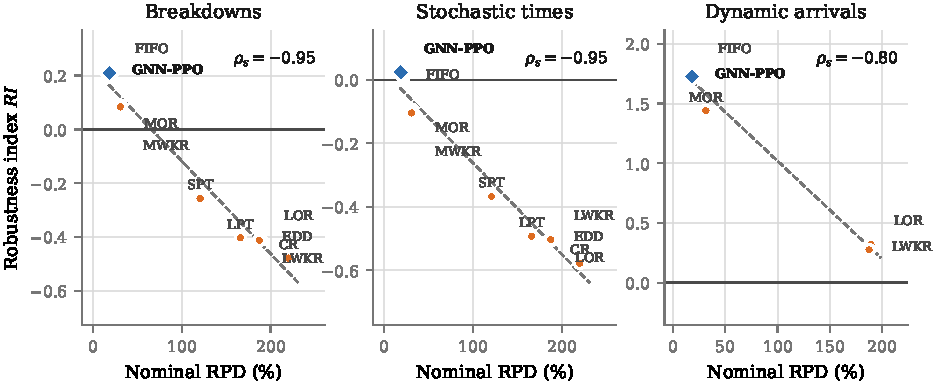
\includegraphics[width=\textwidth]{figures/Fig1_ri_artifact}
  \caption{The robustness index against nominal deviation, aggregated by
  disruption class. Each point is one method. The dashed line is an ordinary
  least-squares fit shown for orientation only; the reported statistic is the
  rank correlation. Methods whose nominal schedules sit furthest from the
  optimum (\textsc{cr}, \textsc{lwkr}, \textsc{lor}, \textsc{edd}) obtain the
  most negative --- conventionally, the most robust --- indices.}
  \label{fig:artifact}
\end{figure*}

\NRINeg{} of the \PropCells{} (method $\times$ instance $\times$ regime) cells in
the corpus --- \PctRINeg{}\% --- have $\RI<0$. By Corollary~\ref{cor:neg} each of these is a case in which the
expected disrupted makespan is below the nominal one, and we verify that the
equivalence holds exactly: in $100\%$ of cells, $\operatorname{sign}(\RI)$ agrees
with $\operatorname{sign}(q-r)$. The critical-ratio rule on \texttt{ft06} under
$A_k=0.90$ is representative --- its nominal makespan of $171$ falls to a mean of
$94.1$ under breakdowns. The rule computes a criticality ratio from due dates
that were synthesised once against nominal durations and are never recomputed as
the realised clock advances, so under disruption its ordering decisions become
progressively less related to the state it is ordering; the resulting near-random
reordering improves on a sequence that was badly chosen to begin with. This is
regression toward the mean, and the index records it as resilience.

\subsection{Rank reversal and the cost of acting on it}\label{sec:res-reversal}

If the index merely added noise, it would still be usable in expectation. It
does not: it induces an ordering that is systematically opposed to the ordering
by realised quality.

\begin{table*}[t]
\caption{Disagreement between the two orderings. $\tau$ is Kendall's rank correlation between the ordering by $\RI$ and the ordering by realised quality. The last three columns give the realised quality of the method the index nominates, that of the method that is actually best, and the penalty incurred by following the index.}\label{tbl:reversal}
\begin{tabular*}{\tblwidth}{@{}LLrllrrr@{}}
\toprule
\multirow{2}{*}{Disruption class} & \multirow{2}{*}{Severity} & \multirow{2}{*}{$\tau$} & \multicolumn{2}{c}{Selected method} & \multicolumn{3}{c}{Realised quality (\%)} \\
\cmidrule(lr){4-5}\cmidrule(l){6-8}
 & & & by $\RI$ & by $\RQ$ & of former & of latter & penalty \\
\midrule
Breakdowns & $A_k=0.95$ & $-0.600$ & CR & MWKR & 46.9 & 23.6 & $+23.3$ \\
 & $A_k=0.90$ & $-0.422$ & CR & MWKR & 63.3 & 34.8 & $+28.5$ \\
 & $A_k=0.80$ & $-0.511$ & CR & \textbf{GNN--PPO} & 90.6 & 64.9 & $+25.7$ \\
Stochastic times & $\sigma=0.10$ & $-0.289$ & CR & MWKR & 30.6 & 12.3 & $+18.4$ \\
 & $\sigma=0.25$ & $-0.378$ & CR & MWKR & 33.7 & 13.7 & $+20.0$ \\
 & $\sigma=0.50$ & $-0.511$ & CR & MWKR & 40.8 & 24.9 & $+15.8$ \\
Dynamic arrivals & $\rho=0.70$ & $-0.400$ & LWKR & \textbf{GNN--PPO} & 268.0 & 230.4 & $+37.6$ \\
 & $\rho=0.85$ & $-0.600$ & LWKR & \textbf{GNN--PPO} & 268.1 & 219.2 & $+48.9$ \\
 & $\rho=0.95$ & $-0.400$ & LWKR & \textbf{GNN--PPO} & 261.1 & 211.7 & $+49.3$ \\
\bottomrule
\end{tabular*}
\end{table*}


Kendall's $\tau$ is negative in all \NRegimes{} regimes (Table~\ref{tbl:reversal},
range \TauMin{} to \TauMax{}), and the two criteria never select the same
method. The per-regime $\tau$ tests are individually significant in only a
minority of regimes --- with at most ten methods each they have little power ---
but the sign is negative without exception, and it is the consistency of that
sign across nine independent regimes, not any single $p$-value, that carries the
claim. The index selects the critical-ratio rule in all \CRWins{} breakdown and
stochastic-time regimes and least-work-remaining in all \LWKRWins{} arrival
regimes. Realised quality selects most-work-remaining or the learned policy. The
penalty for following the index --- the difference in realised quality between
the method it nominates and the method that is actually best --- ranges from
\PenaltyMin{} to \PenaltyMax{} percentage points, with a median of
\PenaltyMedian{}. Figure~\ref{fig:reversal} shows the reversal directly.

\begin{figure*}[t]
  \centering
  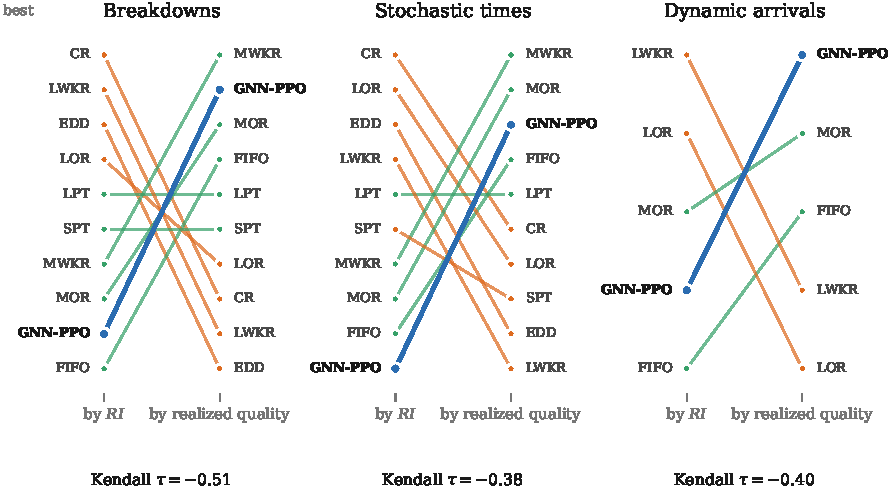
\includegraphics[width=\textwidth]{figures/Fig2_rank_reversal}
  \caption{Ordering by the robustness index (left) against ordering by realised
  quality (right), by disruption class. Lines that fall from left to right are
  methods the index flatters. The learned policy travels from near-worst to
  best; the due-date rules travel in the opposite direction.}
  \label{fig:reversal}
\end{figure*}

\subsection{Realised quality and tail risk}\label{sec:res-rq}

Table~\ref{tbl:axis} gives the full metric panel. Reading the columns against
each other is instructive: the ordering of the $\RI$ column is close to the
reverse of the ordering of the $\RQ$ column, and the nominal-deviation column
explains the former almost entirely.

\begin{table}[t]
\caption{Metric panel by disruption class, methods ordered by realised quality. $r$ is nominal deviation from the certified optimum; $\RI$ the conventional index; $\RQ$ realised quality; $\CVaR_{90}$ its worst-decile mean. All percentages. $^{\star}$ marks the learned policy.}\label{tbl:axis}
\begin{tabular*}{\tblwidth}{@{}Lrrrr@{}}
\toprule
Method & $r$ (\%) & $\RI$ & $\RQ$ (\%) & $\CVaR_{90}$ (\%) \\
\midrule
\multicolumn{5}{@{}l}{\textit{Breakdowns}} \\[2pt]
\quad MWKR & 30.7 & +0.084 & 41.7 & 88.0 \\
\quad \textbf{GNN--PPO}$^{\star}$ & 18.4 & +0.210 & 41.8 & 85.3 \\
\quad MOR & 31.5 & +0.090 & 43.2 & 85.6 \\
\quad FIFO & 21.1 & +0.212 & 46.8 & 89.6 \\
\quad LPT & 165.9 & -0.402 & 57.7 & 107.4 \\
\quad SPT & 120.7 & -0.256 & 64.2 & 122.8 \\
\quad LOR & 189.2 & -0.410 & 65.8 & 130.3 \\
\quad CR & 220.1 & -0.478 & 67.0 & 131.1 \\
\quad LWKR & 187.4 & -0.412 & 68.8 & 134.6 \\
\quad EDD & 187.4 & -0.411 & 69.2 & 129.7 \\
\addlinespace
\multicolumn{5}{@{}l}{\textit{Stochastic times}} \\[2pt]
\quad MWKR & 30.7 & -0.105 & 17.0 & 36.0 \\
\quad MOR & 31.5 & -0.094 & 19.1 & 38.0 \\
\quad \textbf{GNN--PPO}$^{\star}$ & 18.4 & +0.023 & 20.0 & 43.4 \\
\quad FIFO & 21.1 & +0.006 & 21.9 & 49.4 \\
\quad LPT & 165.9 & -0.493 & 33.2 & 59.8 \\
\quad CR & 220.1 & -0.578 & 35.0 & 67.0 \\
\quad LOR & 189.2 & -0.505 & 38.6 & 69.8 \\
\quad SPT & 120.7 & -0.368 & 39.6 & 63.8 \\
\quad EDD & 187.4 & -0.505 & 42.2 & 71.4 \\
\quad LWKR & 187.4 & -0.503 & 42.6 & 74.6 \\
\addlinespace
\multicolumn{5}{@{}l}{\textit{Dynamic arrivals}} \\[2pt]
\quad \textbf{GNN--PPO}$^{\star}$ & 18.4 & +1.728 & 220.4 & 275.1 \\
\quad MOR & 31.5 & +1.441 & 221.1 & 273.4 \\
\quad FIFO & 21.1 & +1.762 & 234.7 & 287.1 \\
\quad LWKR & 187.4 & +0.275 & 265.7 & 307.6 \\
\quad LOR & 189.2 & +0.321 & 266.4 & 310.6 \\
\bottomrule
\end{tabular*}
\end{table}


Under breakdowns the learned policy attains $\RQ=41.8\%$ with
$\CVaR_{90}=85.3\%$ --- the best tail in the panel --- while
\textsc{mwkr} attains a marginally better mean ($41.7\%$) with a worse tail
($88.0\%$). The critical-ratio rule, which the conventional index ranks first,
realises $67.0\%$ with a $131.1\%$ tail. Under stochastic processing times
\textsc{mwkr} leads on both mean and tail, with the policy third. Under dynamic
arrivals the policy leads on the mean and \textsc{mor} on the tail, the two
being close; the absolute magnitudes in this class are large for the reason
given in Section~\ref{sec:framework} and should be read comparatively.
Figure~\ref{fig:rq} displays mean and tail jointly.

\begin{figure*}[t]
  \centering
  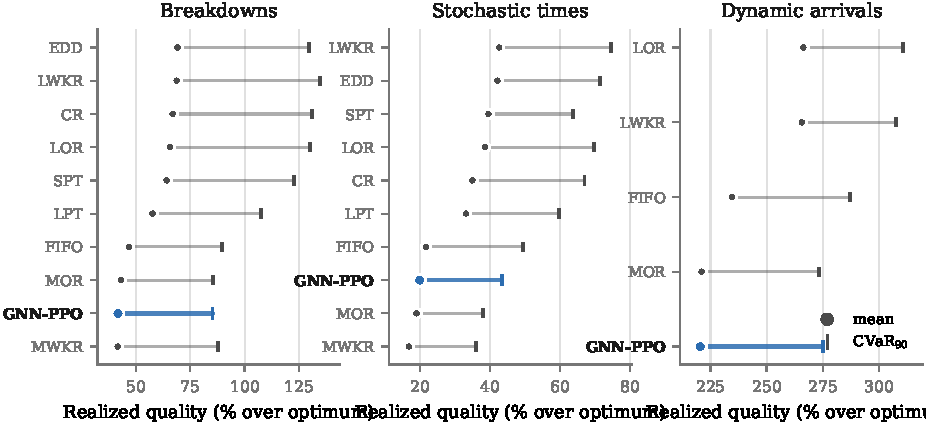
\includegraphics[width=\textwidth]{figures/Fig4_realized_quality}
  \caption{Realised quality by method and disruption class. The circle is the
  mean, the tick the $\CVaR_{90}$, and the segment between them the tail
  exposure. Methods are ordered by mean realised quality.}
  \label{fig:rq}
\end{figure*}

\subsection{Method separation under the corrected metric}\label{sec:res-friedman}

\begin{table*}[t]
\caption{Friedman tests on realised quality with Nemenyi post-hoc, by regime. Blocks are (instance, seed) pairs. The last column records whether the learned policy is statistically indistinguishable from the best-ranked method at the critical difference.}\label{tbl:friedman}
\begin{tabular*}{\tblwidth}{@{}LLrrrlrlrc@{}}
\toprule
Disruption class & Severity & $k$ & $N$ & $\chi^2$ & $p$ & CD & Best-ranked & GNN--PPO rank & Tied \\
\midrule
Breakdowns & $A_k=0.95$ & 10 & 60 & 256.0 & $<10^{-8}$ & 1.75 & MWKR & 2.83 & \checkmark \\
 & $A_k=0.90$ & 10 & 60 & 252.5 & $<10^{-8}$ & 1.75 & \textbf{GNN--PPO} & 2.83 & \checkmark \\
 & $A_k=0.80$ & 10 & 60 & 170.4 & $<10^{-8}$ & 1.75 & \textbf{GNN--PPO} & 3.12 & \checkmark \\
Stochastic times & $\sigma=0.10$ & 10 & 60 & 289.1 & $<10^{-8}$ & 1.75 & MWKR & 3.28 & \checkmark \\
 & $\sigma=0.25$ & 10 & 60 & 267.3 & $<10^{-8}$ & 1.75 & MWKR & 3.15 & \checkmark \\
 & $\sigma=0.50$ & 10 & 60 & 150.6 & $<10^{-8}$ & 1.75 & MWKR & 3.85 & \checkmark \\
Dynamic arrivals & $\rho=0.70$ & 5 & 60 & 183.0 & $<10^{-8}$ & 0.79 & \textbf{GNN--PPO} & 1.62 & \checkmark \\
 & $\rho=0.85$ & 5 & 60 & 200.4 & $<10^{-8}$ & 0.79 & \textbf{GNN--PPO} & 1.57 & \checkmark \\
 & $\rho=0.95$ & 5 & 60 & 190.1 & $<10^{-8}$ & 0.79 & \textbf{GNN--PPO} & 1.57 & \checkmark \\
\bottomrule
\end{tabular*}
\end{table*}


The Friedman null is rejected in every regime with $p\le\FriedmanPMax{}$
(Table~\ref{tbl:friedman}), so the methods are distinguishable on realised
quality everywhere. The learned policy is the top-ranked method in \NRLBest{} of
\NRegimes{} regimes and is not significantly worse than the top-ranked method in
any of the \NRLNotWorse{}.

Under dynamic arrivals the policy takes first rank in all three regimes, at
average ranks of \ArrRankMin{}--\ArrRankMax{} against a critical difference of
\ArrCD{}. It is not, however, separated from the whole field: \textsc{mor}
trails it by only \ArrGapMin{}--\ArrGapMax{} rank points, well inside the
critical difference, so the correct statement is that the policy and
\textsc{mor} are statistically tied at the top while \textsc{fifo},
\textsc{lwkr} and \textsc{lor} fall outside it. Figure~\ref{fig:cd} shows the
critical-difference diagrams, in which the clique bar spans exactly that pair.
The same reading applies in the other six regimes, where the policy's clique
also contains \textsc{mwkr}, \textsc{mor} and \textsc{fifo}: nowhere in this
corpus does the learned policy separate from every rule.

\begin{figure*}[t]
  \centering
  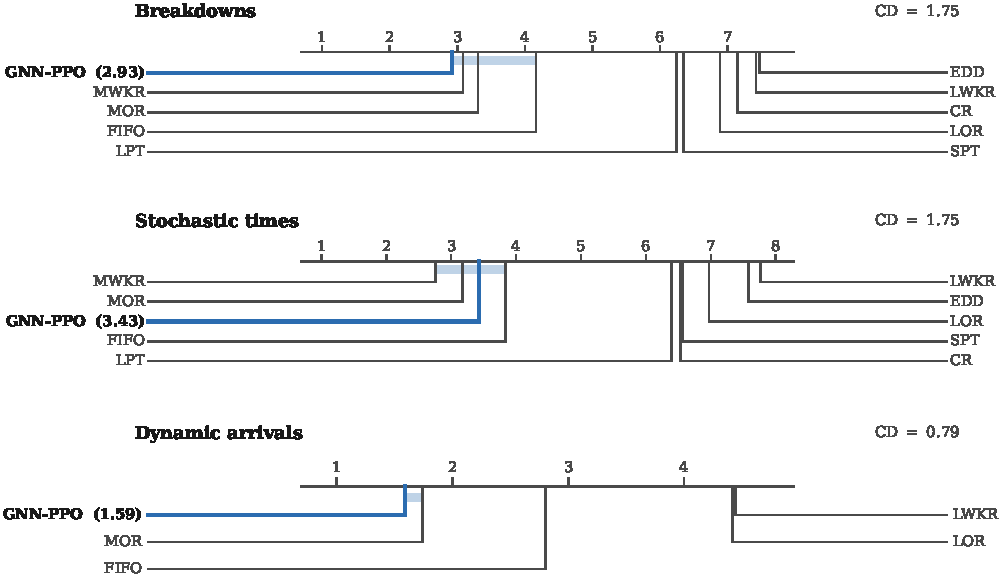
\includegraphics[width=\textwidth]{figures/Fig3_critical_difference}
  \caption{Critical-difference diagrams on realised quality, one per disruption
  class. Methods joined by the shaded bar are not distinguishable from the
  best-ranked method at $\alpha=0.05$.}
  \label{fig:cd}
\end{figure*}

\subsection{Comparator sensitivity}\label{sec:res-comparators}

Table~\ref{tbl:comparators} evaluates the three comparators of
Section~\ref{sec:comparators} on the \NInstances{}-instance nominal corpus.

\begin{table*}[t]
\caption{The same policy against three definitions of ``best dispatching rule''. Deviations are relative percentage deviation from the certified optimum; the difference column is the median paired difference in percentage points, with Wilcoxon $z$, $p$ and rank-biserial effect size over the paired instances; $N=43$ for the learned-policy rows and $N=40$ where exact ties are dropped, as the $n$ column records.}\label{tbl:comparators}
\begin{tabular*}{\tblwidth}{@{}LrLrrrrlrl@{}}
\toprule
Comparator & Its RPD & Method & Its RPD & Median diff. & $n$ & $z$ & $p$ & $r_{rb}$ & Verdict \\
\midrule
$\mathrm{PDR}_{\mathrm{global}}$ & 251.4 & \textbf{GNN--PPO} & 24.8 & $+233.4$ & 43 & -5.71 & $1.1\times10^{-8}$ & $+1.000$ & \textsc{wins} \\
 & 251.4 & GA & 5.5 & $+251.5$ & 43 & -5.71 & $1.1\times10^{-8}$ & $+1.000$ & \textsc{wins} \\
 & 251.4 & CP-SAT & 0.0 & $+254.6$ & 43 & -5.71 & $1.1\times10^{-8}$ & $+1.000$ & \textsc{wins} \\
$\mathrm{PDR}_{\mathrm{family}}$ & 148.1 & \textbf{GNN--PPO} & 24.8 & $+132.4$ & 43 & -5.71 & $1.1\times10^{-8}$ & $+1.000$ & \textsc{wins} \\
 & 148.1 & GA & 5.5 & $+144.3$ & 43 & -5.71 & $1.1\times10^{-8}$ & $+1.000$ & \textsc{wins} \\
 & 148.1 & CP-SAT & 0.0 & $+152.1$ & 43 & -5.71 & $1.1\times10^{-8}$ & $+1.000$ & \textsc{wins} \\
$\mathrm{PDR}_{\mathrm{oracle}}$ & 19.0 & \textbf{GNN--PPO} & 24.8 & $-7.6$ & 43 & -4.11 & $4.0\times10^{-5}$ & $-0.719$ & \textsc{loses} \\
 & 19.0 & GA & 5.5 & $+11.5$ & 40 & -5.51 & $3.6\times10^{-8}$ & $+1.000$ & \textsc{wins} \\
 & 19.0 & CP-SAT & 0.0 & $+21.1$ & 40 & -5.51 & $3.6\times10^{-8}$ & $+1.000$ & \textsc{wins} \\
\bottomrule
\end{tabular*}
\end{table*}


The verdict on the learned policy depends entirely on which comparator is
chosen. Against the mean of the nine rules it wins by \CompGlobal{} percentage
points; against the best rule per family, by \CompFamily{}; against the
per-instance oracle, it \emph{loses} by \CompOracle{}. All three differences are
significant over $N=\NInstances{}$ paired instances ($p\le\CompPMax{}$; exact
values in Table~\ref{tbl:comparators}). A paper
reporting only the first would claim a decisive win; one reporting only the
third, a decisive loss. Both would be describing the same runs.
Figure~\ref{fig:comparators} shows the three distributions.

\begin{figure*}[t]
  \centering
  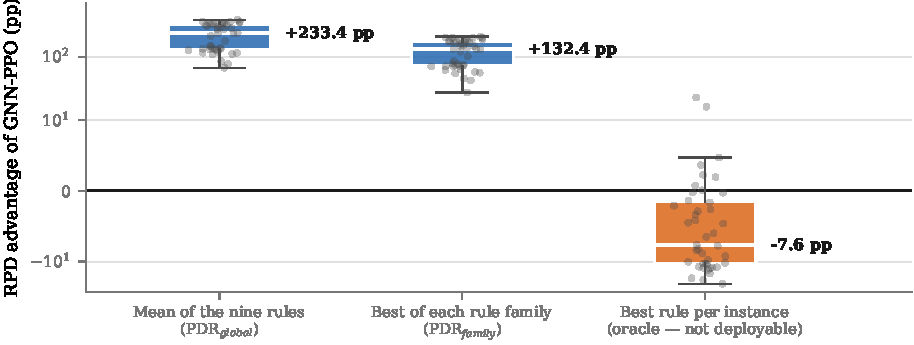
\includegraphics[width=\textwidth]{figures/Fig6_comparator_sensitivity}
  \caption{Advantage of the learned policy over three definitions of the
  dispatching-rule baseline, per instance. The vertical scale is symmetric-log.
  The oracle comparator is included for calibration and is not deployable.}
  \label{fig:comparators}
\end{figure*}

\subsection{What optimality buys under disruption}\label{sec:res-exact}

A supplementary comparison bears on the motivating claim of the DRL-scheduling
literature. On \texttt{ft06} under breakdowns at $A_k=0.90$, CP-SAT and the
genetic algorithm both reach the proven optimum nominally ($r=0$). Executed with
right-shift repair over five shared disruption seeds, they realise \QCpsat{}\%
and \QGa{}\% above the optimum respectively --- against \QMor{}\% for
\textsc{mor}, \QMwkr{}\% for \textsc{mwkr} and \QRl{}\% for the learned policy.
The paired differences between the policy and either the exact or the
metaheuristic method are not significant at this sample size ($p=\PRlCpsat{}$
and $p=\PRlGa{}$; one seed produces an exact tie for all three methods, leaving
$n=\NEffOffline{}$ non-zero differences). The genetic algorithm consumes
\WallGa{}~s per instance and CP-SAT \WallCpsat{}~s, against \WallRl{}~s for the
policy's full rollout.

The reading we take from this is deliberately cautious. Five seeds on one
instance in one regime is a descriptive observation, not a test, and we report
it as such. What it does suggest is that nominal optimality is largely dissipated
by right-shift execution, which is the substantive question the robustness index
was introduced to answer and which realised quality answers directly.

% ===========================================================================
\section{Discussion}\label{sec:discussion}

\subsection{What the index was measuring}

Proposition~\ref{prop:ri} shows that $\RI$ is a normalised difference between
realised and nominal quality, and Section~\ref{sec:res-artifact} shows that in
practice the nominal term dominates. The index is therefore best understood not
as a robustness measure that happens to be noisy but as a measure of a different
quantity --- roughly, how much headroom a method left itself --- reported under
a name that invites the wrong interpretation. A method with no headroom, because
it scheduled well, cannot score well on it.

This does not make the underlying question empty. ``How much of its planned
quality does a method retain under realisation?'' is a real and important
question, and the difference $q-r$ answers it on an interpretable scale.
What must be abandoned is the normalisation by $\Cmax^{\text{nom}}$, and with
it the practice of comparing $\RI$ across methods.

\subsection{Implications for reported results}

We are not in a position to re-analyse other authors' data, and we make no claim
about the correctness of any specific published result. What
Proposition~\ref{prop:ri} does establish is conditional and, we think,
consequential: wherever a comparison of methods rests on an index of the form of
Definition~\ref{def:ri}, and wherever the compared methods differ appreciably in
nominal quality, the reported ordering is confounded by that difference in a
known direction and by a computable amount. Since learned policies and
dispatching rules routinely differ by a factor of several in nominal deviation
--- on the two disruption instances of this corpus, \NomRlTwo{}\% for the
learned policy against \NomCrTwo{}\% for the critical-ratio rule, and
\NomRlAll{}\% against \NomCrAll{}\% over the full \NInstances{}-instance
nominal set --- the condition is not a corner case.

The remedy is cheap. Realised quality is computable from records that any such
study already possesses, provided a certified optimum or an accepted bound is
available for the nominal instance; it requires no re-execution. We would
encourage reporting $r$, $q$ and $q-r$ together, and reserving robustness
language for the last of the three.

\subsection{A reporting protocol}

The audit suggests four requirements, none onerous.
\begin{enumerate}[(1)]
\item Grade disrupted performance against a reference external to the method:
a certified optimum where one exists, otherwise a fixed bound shared by all
methods and named as such.
\item Report nominal deviation alongside any robustness quantity, so that
readers can perform the decomposition of Proposition~\ref{prop:ri} themselves.
\item Report a tail statistic, not only a mean.
\item Name the comparator. If the claim is against ``the best dispatching
rule'', state which of the three constructions of
Section~\ref{sec:comparators} is meant, and prefer reporting more than one.
\end{enumerate}

\subsection{Threats to validity}\label{sec:threats}

We state the limits of this study plainly, because several of them bound the
conclusions materially.

\paragraph{Instance breadth in the disruption grid.} The \NRegimes{} regimes are
executed on two instances, \texttt{ft06} and \texttt{la01}. The analytic result
of Proposition~\ref{prop:ri} is instance-independent, and the empirical
correlations are computed across methods rather than across instances, so the
audit's central claim does not rest on instance breadth. The method-level
findings of Section~\ref{sec:res-friedman} do, and should be read as holding for
these two instances and this disruption model rather than as a general ranking.

\paragraph{Equivalence from non-rejection.} A Nemenyi non-rejection is a failure
to distinguish, not a demonstration of equivalence. With $k=10$ and $N=60$ the
critical difference is $1.75$ on a rank scale of $1$ to $10$, which is wide; the
statement that the policy is ``not significantly worse'' should be read with that
width in mind rather than as a claim of parity.

\paragraph{Training seeds.} The learned policy is a single trained checkpoint.
Its position in Table~\ref{tbl:friedman} therefore carries no estimate of
training variance, and the reinforcement-learning reproducibility literature is
emphatic that this variance can be large \citep{henderson2018,agarwal2021}.
Multi-seed training infrastructure is implemented and reported in the
accompanying repository, but the multi-seed campaign had not completed at the
time of writing and no multi-seed number is claimed here.

\paragraph{Method coverage under disruption.} The nine-regime grid compares the
learned policy against nine dispatching rules in six regimes and four in the
other three (Section~\ref{sec:execution}). CP-SAT and the genetic algorithm enter
only through the descriptive comparison of Section~\ref{sec:res-exact}, at one
instance, one regime and five seeds. Consequently, wherever this paper says the
policy is not significantly worse than the best method, the comparison set is the
dispatching rules in that regime, not the exact and metaheuristic solvers ---
and in the single regime where those solvers were run they finish ahead of the
policy (\QCpsat{}\% and \QGa{}\% against \QRl{}\%), though not significantly so
at $n=\NEffOffline{}$. A full offline-method arm across the grid is the natural
next experiment and would sharpen Section~\ref{sec:res-exact} from an
observation into a test.

\paragraph{Rule coverage under arrivals, and why it is not conservative.} Five
of the ten methods are compared in the arrival regimes, for the reasons given in
Section~\ref{sec:execution}. This cuts in two directions and we want to be
explicit about both. For the measurement claim it is close to neutral: the
excluded set spans the range: it contains the two rules with the worst nominal
schedules (\textsc{cr}, \textsc{edd}) and also the rule with the second best
(\textsc{mwkr}, at \NomMwkrTwo{}\%), so it does not manufacture the negative
correlation --- which in any case rests on the \NConfRegimes{} ten-method
regimes. For the claim about
the learned policy it is \emph{anti}-conservative: \textsc{mwkr}, which
outranks the policy in five of the six non-arrival regimes, is excluded, so the policy's first rank
under arrivals is a first rank in a weakened field. We therefore do not treat
the arrival result as the strongest evidence for the policy, and a reader who
discounts it entirely is left with the measurement argument, which does not
depend on it.

\paragraph{Reference validity under arrivals.} As noted in
Section~\ref{sec:framework}, $\RQ$ under dynamic arrivals is referenced to the
optimum of the nominal instance rather than of the realised one. Comparisons
within a regime remain valid; absolute magnitudes there are not optimality gaps.

\paragraph{Post-hoc status of the re-measurement.} The measurement audit was not
pre-registered. It was prompted by an examination of the metric and is reported
as post-hoc analysis of a frozen corpus. No datum was altered, and the
pre-registered verdicts computed on the original metric stand as recorded in the
accompanying materials.

% ===========================================================================
\section{Conclusion}\label{sec:conclusion}

The robustness index that dominates evaluation of dynamic scheduling under
disruption normalises a method's degradation by its own nominal makespan. We
proved that this makes the index strictly decreasing in nominal deviation at
fixed realised performance, so that the worse a method's plan, the more robust
it appears, and that a negative index --- widely read as exceptional resilience
--- is the signature of a plan poor enough for perturbation to improve it. In a
pre-registered corpus of \NRunsDisrupted{} disrupted executions across
\NRegimes{} regimes, the index is negatively rank-correlated with nominal
deviation everywhere and at $\rho_s\in[\RhoConfMin{},\RhoConfMax{}]$ in the
\NConfRegimes{} regimes with a ten-method field, it orders methods opposite to
realised quality in every regime, and following it costs up to \PenaltyMax{}
percentage points of deviation from the optimum.

Realised quality --- the deviation of the executed makespan from a certified
optimum --- together with a $\CVaR_{90}$ tail and an explicitly named
dispatching comparator, repairs the comparison at the cost of re-measurement
alone. Re-measured this way, the heterogeneous GNN--PPO policy is not
significantly worse than the best-ranked dispatching rule in any of the
\NRegimes{} regimes and takes first rank in \NRLBest{}, including all three
dynamic-arrival regimes, where the value of deciding online is greatest --- in
every case tied with \CliqueArr{} rule under arrivals and \CliqueOther{}
elsewhere, rather than separated from the field. The
conventional index places the same policy near the bottom of the same runs.

The wider point is methodological. A metric whose denominator is chosen by the
method being graded cannot support a comparison between methods, and the
scheduling literature has a well-established external reference available in the
certified optima of its standard benchmarks. Using it costs nothing and settles
the question the index was introduced to answer.

% ===========================================================================
\section*{CRediT authorship contribution statement}

\textbf{Joseph Javier Sánchez Acuña:} Conceptualization, Methodology, Software,
Formal analysis, Investigation, Data curation, Writing -- original draft,
Writing -- review \& editing, Visualization.

\section*{Declaration of competing interest}

The author declares no known competing financial interests or personal
relationships that could have appeared to influence the work reported in this
paper.

\section*{Data availability}

The source code, the pre-registration document, the raw per-run records
underlying every table and figure, and the analysis scripts that regenerate them
are available in the accompanying public repository. Every number reported in
Section~\ref{sec:results}, including the identity audit of
Section~\ref{sec:framework} and the offline-method comparison of
Section~\ref{sec:res-exact}, is produced by those scripts from those records.

\appendix

\section{Research programme}\label{app:gantt}

Figure~\ref{fig:gantt} sets out the schedule of the research programme from
which the corpus arises, including the point at which the pre-registration was
frozen and the point at which the confirmatory campaign closed. The measurement
audit reported in this paper follows both.

\begin{figure*}[t]
  \centering
  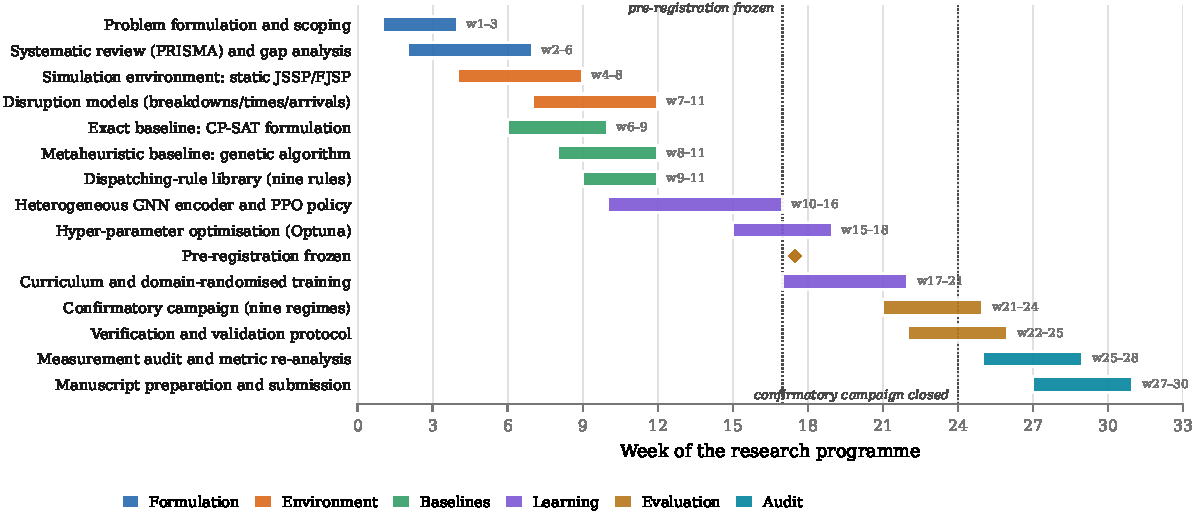
\includegraphics[width=\textwidth]{figures/Fig5_gantt}
  \caption{Schedule of the research programme. The diamond marks the
  pre-registration freeze, after which no hypothesis, threshold, instance set or
  statistical test was altered. The measurement audit and the re-analysis
  reported here occupy the final phase and are post-hoc with respect to that
  freeze.}
  \label{fig:gantt}
\end{figure*}

\printcredits

\bibliographystyle{cas-model2-names}
\bibliography{refs}

\end{document}
